\setcounter{chapter}{8}
\chapter{Forces des acides et bases}

\section{L'autoprotolyse de l'eau}
\subsection{L'eau, une espèce amphotère}
\blocrouge{Définition}{L'eau peut à la fois capter un ion $H^+$ ou en céder un. On dit que $H_2O$ est une espèce \trou{amphotère}}

Couples de l'eau : $H_3O^+/H_2O$ et $H_2O/HO^-$\\
L'eau peut donc être le seul réactif d'une réaction acide base appelée \textbf{l'autoprotolyse} de l'eau :

\begin{center}
$\trou{H_2O(l) + H_2O(l) \rightleftharpoons H_3O^+(aq) +HO^{-}(aq)}$	
\end{center}

\subsection{Le produit ionique de l'eau}

%Le pH de l'eau pure est égal à 7, ce qui signifie que $\rm [H_3O^+]=\trou{\SI{e-7}{\mole\per\liter}}$. Il y a donc présence d'ions $\rm[H_3O^+]$ dans l'eau. Ils proviennent de la réaction \trou{2\chemfig{H_2O} \chemrel{<>} \chemfig{H_3O^+} \chemsign+ \chemfig{HO^{-}}}\\
\blocrouge{Définition}{Pour toute solution aqueuse à l'équilibre chimique, on a $$\trou{\dfrac{\rm[H_3O^+]_{eq}\times[HO^{-}]_{eq}}{(c^o)^2}=10^{-14}=Ke}$$
Ke est appelé le produit ionique de l'eau. Par définition: $c^0=\SI{1}{\mol\per\liter}$. On y associe le pKe tel que $\rm pKe=-\log Ke=14$}


\section{Echelle des pH}

\subsection{Applications}
\etiquette{Situation 1}
On considère une solution dont le pH est égal à 3,5. 
\begin{enumerate}
	\item Cette solution est-elle acide, basique ou neutre ?\trou{cette solution est acide}
	\item Calculer $\rm[H_3O^+]_{eq}$ et $\rm[HO^-]_{eq}$. Comparer ces deux valeurs.
\end{enumerate}

\trou{$\rm[H_3O^+]_{eq}=10^{-3,5}=\SI{3,2e-4}{\mole\per\liter}$\\
$\rm[HO^-]_{eq}=\frac{Ke(c^0)^2}{[H_3O^+]_{eq}}=\frac{10^{-14}}{\num{3,2e-4}}=\SI{3,1e-11}{\mole\per\liter}$\\
On remarque que la concentration en ions $\rm H_3O^+$ est très supérieure à celle des ions $\rm HO^-$}

\etiquette{Situation 2} On considère  une solution de soude telle que $\rm[HO^-]_{eq}=\SI{1,0e-3}{\mole\per\liter}$.\\ Calculer $\rm[H_3O^+]_{eq}$ puis le pH\\
\trou{$\rm[H_3O^+]_{eq}=\frac{Ke(c^0)^2}{[HO^-]_{eq}}=\frac{10^{-14}}{\num{1,0e-3}}=\SI{1,0e-11}{\mole\per\liter}$\\
$\rm pH=-\log \num{1,0e-11}=11$}


\subsection{Échelle des pH}
\blocrouge{Définition}{
\includegraphics[scale=.80]{figures/acide_base/echelle_pH}

Solution neutre : \trou{$\rm[H_3O^+]_{eq}=[HO^-]_{eq}$ et $\rm pH=7$}\\
Solution acide : \trou{$\rm[H_3O^+]_{eq}>[HO^-]_{eq}$ et $\rm pH<7$}\\
Solution basique :\trou{ $\rm[H_3O^+]_{eq}<[HO^-]_{eq}$ et $\rm pH>7$}\\
}

\section{Réaction d'un acide ou d'une base avec l'eau}
\subsection{Cas des acides faibles - Réaction de l'acide éthanoïque avec l'eau}
\blocgris{Expérience}{
Nous introduisons $\SI{5,0e-4}{\mole}$ d'acide éthanoïque pur dans un $\SI{50}{\milli\liter}$ d'eau. Nous mesurons le pH de la solution, et nous trouvons pH=3,4.
}

Remplir le tableau d'évolution du système et en déduire si la transformation de l'acide éthanoïque avec l'eau est totale. : \\
\small
\begin{tabular}{|p{3cm}|p{1.5cm}|p{3cm}|p{1.2cm}|p{2cm}|p{2cm}|}
\hline 
  \multicolumn{2}{|c!{\protect\makebox[0cm]{:}}}{\textbf{Equation de la réaction}} &
 \multicolumn{1}{c!{\protect\makebox[0cm]{+}}}{%
      $\trou{\rm{CH_3COOH(aq)}}$} &
       \multicolumn{1}{c!{\protect\makebox[0cm]{ $\rightarrow$ }}}{%
      $\trou{\rm{H_2O(l)}}$} 
			&\multicolumn{1}{c!{\protect\makebox[0cm]{ + }}}
			{$\trou{\rm{CH_3COO^-(aq)}}$} 
			&\multicolumn{1}{c|}{
			$\trou{\rm{H_3O^+(aq)}}$} 
\tabularnewline


\hline 
Etat initial&
$x=0$&\trou{\num{5,0e-4}}
&\trou{excès}
&\trou{0}
&\trou{0}

\tabularnewline
\hline 
Etat intermédiaire&
$x$&\trou{\num{5,0e-4}-x}
&\trou{excès}
&\trou{x}
&\trou{x}

\tabularnewline
\hline 
Etat final= \textbf{Equilibre Chimique}&
$x=x_{f}$&$\rm \trou{\num{5,0e-4}-x_f}$
&\trou{excès}
&$\rm \trou{x_f}$
&$\rm \trou{x_f}$

\tabularnewline
\hline 
Etat final si la transformation était totale&
$x=x_{max}$&$\trou{\num{5,0e-4}-x_{max}}$
&\trou{excès}
&$\rm \trou{x_{max}}$
&$\rm \trou{x_{max}}$
\tabularnewline
\hline
\end{tabular}
\normalsize


$\trou{\rm x_f=[H_3O^+]_{eq} \times V=10^{-3,4}\times c^0 \times 0,050=\SI{2,0e-5}{\mol}}$\\

\etiquetterouge{Réfléchir!}
Ici $\rm x_f$ est différent de $\rm x_{max}$, ce qui signifie que la réaction n'est pas totale. La réaction atteint son état final (plus de consommation de réactif) alors que les deux réactifs sont encore présents. On dit que l'équilibre chimique est atteint. L'avancement à l'état final est donc inférieur à $x_{max}$ qui correspond à la consommation du réactif limitant.


\subsection{Cas des acides forts - Réaction de l'acide nitrique avec l'eau}

\blocgris{Expérience}{
Nous introduisons $\SI{5,0e-4}{\mole}$ d'acide nitrique pur dans un $\SI{50}{\milli\liter}$ d'eau. Nous mesurons le pH de la solution, et nous trouvons pH=2.
}


Remplir le tableau d'évolution du système et en déduire si la transformation de l'acide nitrique avec l'eau est totale. : 

\begin{tabular}{|p{3cm}|p{2cm}|p{3cm}|p{2cm}|p{1.5cm}|p{1.5cm}|}
\hline 
  \multicolumn{2}{|c!{\protect\makebox[0cm]{:}}}{\textbf{Equation de la réaction}} &
 \multicolumn{1}{c!{\protect\makebox[0cm]{+}}}{%
      $\trou{\rm HNO_3}$} &
       \multicolumn{1}{c!{\protect\makebox[0cm]{ $\rightarrow$ }}}{%
      $\trou{\rm{H_2O(l)}}$} 
			&\multicolumn{1}{c!{\protect\makebox[0cm]{ + }}}
			{$\trou{\rm NO_3^-}$} 
			&\multicolumn{1}{c|}{
			$\trou{\rm H_3O^+}$} 
\tabularnewline


\hline 
Etat initial&
$x=0$&\trou{\num{5,0e-4}}
&\trou{excès}
&\trou{0}
&\trou{0}

\tabularnewline
\hline 
Etat intermédiaire&
$x$&\trou{\num{5,0e-4}-x}
&\trou{excès}
&\trou{x}
&\trou{x}

\tabularnewline
\hline 
Etat final&
$x=x_{f}$&$\rm \trou{\num{5,0e-4}-x_f}$
&\trou{excès}
&$\rm \trou{x_f}$
&$\rm \trou{x_f}$

\tabularnewline
\hline 
Etat final si la transformation était totale&
$x=x_{max}$&$\trou{\num{5,0e-4}-x_{max}}$
&\trou{excès}
&$\rm \trou{x_{max}}$
&$\rm \trou{x_{max}}$
\tabularnewline
\hline
\end{tabular}


\trou{$\rm x_f=[H_3O^+]_{eq} \times V=10^{-2}\times c^0 \times 0,050=\SI{5,0e-4}{\mole}$\\
On remarque que $\rm x_f= x_{max}$, ce qui signifie que la réaction est totale..}
\subsection{Conclusion}

\etiquetterouge{Acide fort ou acide faible ?}


 Lorsque l'on introduit un acide dans l'eau, deux cas sont possibles : 
\begin{enumerate}
\item
Sa réaction avec l'eau est totale.\\On parle alors d'acide fort.\\On écrit : $$\trou{HA(aq) + H_2O(l) \longrightarrow H_3O^+(aq) + A^{-}(aq)}$$
C'est le cas de l'acide nitrique : $$ HNO_3(aq)+H_2O(l) \longrightarrow H_3O^+(aq) + NO_3^{-}(aq)$$


\item 
Sa réaction avec l'eau n'est pas totale.\\
On parle alors d'acide faible.\\On écrit :
$$HA(aq) + H_2O(l) \rightleftharpoons \trou{H_3O^+(aq) }+ \trou{A^{-}(aq) }$$
C'est le cas de l'acide éthanoïque :
$$ CH_3COOH(aq) + H_2O(l) \rightleftharpoons \trou{H_3O^+(aq) + CH_3COO^{-}(aq)}$$

\end{enumerate}

\subsection{Réaction d'une base avec l'eau}

On raisonne par analogie à ce que l'on a appris sur la réaction entre un acide et l'eau.\\
Lorsque l'on introduit une base dans l'eau, deux cas sont possibles : 
\begin{itemize}
\item
Sa réaction avec l'eau est totale.\\On parle alors de \trou{ base forte}.\\On écrit :  $$ A^-(aq) + H_2O(l) \longrightarrow AH(aq) + HO^{-}(aq)$$
\item 
Sa réaction avec l'eau n'est pas totale.\\
On parle alors de \trou{base faible}.\\On écrit :  $$ A^-(aq) + H_2O(l)\rightleftharpoons  AH(aq) + HO^{-}(aq)$$
\end{itemize}

\section{Calculer le pH des solutions d'acide fort et de base forte}

\etiquette{Situation} Lors de la préparation d'une solution d'acide ou de base, il y a eu réaction chimique entre le soluté (l'acide ou la base) et le solvant ($H_2O$).

L'état initial est le moment où l'on apporte une certaine quantité de matière de soluté. Celle-ci est notée $n_0$ dans la suite. 
Lorsque l'on prépare un volume V de solution à partir de $n_0$, on obtient une solution de concentration en soluté apporté C tel que $$C=\frac{n_0}{V}$$


\subsection{Cas d'un Acide FORT}

On considère une solution d'acide HA de concentration $\rm C$ et de volume V. \\
\begin{tabular}{|l|p{2cm}|p{2cm}|p{2cm}|p{2cm}|p{2cm}|}
\hline 
  \multicolumn{2}{|c!{\protect\makebox[0cm]{:}}}{\textbf{Equation de la réaction}} &
 \multicolumn{1}{c!{\protect\makebox[0cm]{+}}}{%
      $\trou{\rm HA}$} &
       \multicolumn{1}{c!{\protect\makebox[0cm]{ $\rightarrow$ }}}{%
      $\trou{\rm{H_2O(l)}}$} 
			&\multicolumn{1}{c!{\protect\makebox[0cm]{ + }}}
			{$\trou{\rm A^-}$} 
			&\multicolumn{1}{c|}{
			$\trou{\rm H_3O^+}$} 
\tabularnewline


\hline 
Etat initial&
$x=0$&\trou{$\rm CV= n_0$}
&\trou{excès}
&\trou{0}
&\trou{0}

\tabularnewline
\hline 
Etat intermédiaire&
$x$&\trou{$\rm CV-x$}
&\trou{excès}
&\trou{x}
&\trou{x}


\tabularnewline
\hline 
Etat final&
$x=x_{max}$&$\trou{CV-x_{max}}$
&\trou{excès}
&$\rm \trou{x_{max}}$
&$\rm \trou{x_{max}}$
\tabularnewline
\hline
\end{tabular}\\
La réaction est totale donc on obtient $\rm x_{max}=\trou{CV = n_0 = n(H_3O^+)_{eq}}$.\\
On a alors $\trou{\rm [H_3O^+]_{eq}=\frac{CV}{V}=C}$ et $\rm pH=-\log \dfrac{C}{c^0}$

\blocrouge{Conclusion}{
Le pH d'une solution d'acide fort est tel que $$\trou{\rm pH=-\log \dfrac{C}{c^0}}$$ avec $\rm C$ la concentration en acide de la solution.}


\subsection{Cas d'une base FORTE}
On considère une solution de base forte notée $\rm A^-$ de concentration $\rm C$ et de volume V. \\
\begin{tabular}{|p{3cm}|p{2cm}|p{2cm}|p{2cm}|p{2cm}|p{2cm}|}
\hline 
  \multicolumn{2}{|c!{\protect\makebox[0cm]{:}}}{\textbf{Equation de la réaction}} &
 \multicolumn{1}{c!{\protect\makebox[0cm]{+}}}{%
      $\trou{\rm A^-}$} &
       \multicolumn{1}{c!{\protect\makebox[0cm]{ $\rightarrow$ }}}{%
      $\trou{\rm{H_2O(l)}}$} 
			&\multicolumn{1}{c!{\protect\makebox[0cm]{ + }}}
			{$\trou{\rm AH}$} 
			&\multicolumn{1}{c|}{
			$\trou{\rm HO^-}$} 
\tabularnewline


\hline 
Etat initial&
$x=0$&\trou{$\rm CV = n_0$}
&\trou{excès}
&\trou{0}
&\trou{0}

\tabularnewline
\hline 
Etat intermédiaire&
$x$&$\trou{\rm CV-x}$
&\trou{excès}
&\trou{x}
&\trou{x}


\tabularnewline
\hline 
Etat final &
$x=x_{max}$&$\trou{CV-x_{max}}$
&\trou{excès}
&$\rm \trou{x_{max}}$
&$\rm \trou{x_{max}}$
\tabularnewline
\hline
\end{tabular}

La réaction est totale donc $x_f=x_{max}=n_0=C\times V$ \\
A l'état final, on a $\trou{\rm [HO^-]=C}$ et $[H_3O^+]=\frac{Ke}{C}\times (c^0)^2$ et $\dfrac{[H_3O^+]}{c^0}=\frac{Ke}{C}\times (c^0)$ .\\On a donc $\trou{-\log \dfrac{[H_3O^+]}{c^0}} =-\log Ke + \log \dfrac{C}{c^0}$ et $\rm pH=pKe+\log \dfrac{C}{c^0}$

\blocrouge{Conclusion}{
Le pH d'une solution de base forte est tel que $\rm pH=pKe+\log \dfrac{C}{c^0}$ avec $\rm C$ la concentration en base de la solution.
}



\section{Force d'un acide}
\subsection{Taux d'avancement}

\blocrouge{Définition}{ Pour indiquer l'aspect total ou limité d'une réaction on calcule le taux d'avancement $$\tau=\dfrac{x_f}{x_{max}}$$}

Si $\tau<1$ alors \trou{la réaction n'est pas totale}. Si $\tau=1$ alors \trou{la réaction est totale.}

Plus le taux d'avancement de la réaction d'un acide avec l'eau est proche de 1 plus cet acide se comporte comme un acide fort. Même raisonnement pour une base.
\subsection{Constante Ka}

\blocrouge{Définitions}{
Soit un couple $\rm HA(aq)/A^-(aq)$ dont l'acide réagit avec l'eau selon la réaction d'équation\\
$$\trou{HA(aq)} + \trou{H_2O(l)} \rightleftarrows H_3O^+(aq) + A^{-}(aq)$$

La constante d'acidité notée Ka du couple est définie par :\\
$$\rm Ka=\trou{\frac{[A^-]_{eq}\times[H_3O^+]_{eq}}{[HA]_{eq}\times c^0}}$$\\
Avec $\rm[A^-]_{eq}$,$\rm[H_3O^+]_{eq}$et$\rm[HA]_{eq}$ les valeurs des  concentrations lorsque le système a atteint son état d'équilibre.\\
On définit également le pKa tel que $\rm pKa=\trou{-\log Ka}$ et par conséquent, $\rm Ka=\trou{10^{-pKa}}$
}

Quelques exemples : \\
\begin{tabular}{|c|c|c|}
\hline
Couple Acide/Base &Ka&pKa\\
\hline
$\rm CH_3COOH/CH_3COO^-$&$\rm \trou{10^{-4,8}}$&4,8\\
\hline
$\rm HCOOH/HCOO^-$&$\rm10^{-3,8}$&\trou{3,8}\\
\hline
$\rm NH_4^+/NH_3$&$\rm \trou{10^{-9,2}}$&9,2\\
\hline
\end{tabular}
\blocgris{Technique importante}{ Comment prévoir la composition chimique d'une solution d'acide connaissant sa concentration et son Ka ?\\
On considère une solution d'acide méthanoïque de concentration égale à $c=\SI{1,0e-2}{\mole\per\liter}$. A partir de la valeur du Ka, retrouver la valeur des concentrations de toutes les espèces chimiques présentes à l'équilibre.
}



\subsection{Classement des acides}
\begin{minipage}{0,65\linewidth}
Un acide est d'autant plus fort que le taux d'avancement de sa réaction avec l'eau est \trou{grand}.\\
$\rm Ka=\trou{\frac{[A^-]_{eq}\times[H_3O^+]_{eq}}{[HA]_{eq}\times c^0}}$\\
Donc, plus un acide est fort, plus :
\begin{itemize}
\item$ [A^-]_{eq}$ sera \trou{élevée}
\item$ [H_3O^+]_{eq}$ sera \trou{élevée}
\item $ [HA]_{eq}$ sera \trou{faible}
\end{itemize}
On en déduit, que plus un acide est fort (et plus sa base conjuguée est faible) plus sa constante d'acidité Ka est \trou{grande}, et par conséquent, plus son pKa est \trou{faible}.
\end{minipage}
\begin{minipage}{0,4\linewidth}
\begin{center}
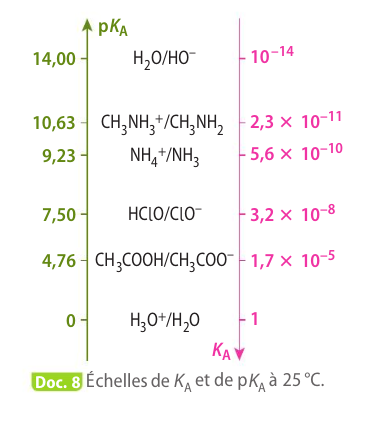
\includegraphics[scale=0.4]{figures/acide_base/fig_pka}
\end{center}
\end{minipage}


\blocrouge{Conclusion}{
Plus la constante d'acidité Ka d'un couple acide-base $AH/A^-$ est grande, plus son pKa est \trou{petit}, plus la force de l'acide AH est \trou{élevée} et plus la force de la base $A^-$ est \trou{faible}.}

\subsection{Diagramme de prédominance}
\etiquetterouge{Définition}\\
Une espèce est prédominante devant une autre espèce si \trou{sa concentration en solution est plus grande que celle de l'autre espèce.}
\\
Afin d'identifier la prédominance d'une espèce d'un couple acide base connaissant son pH et son pKa, nous allons établir la relation entre le pH et le pKa d'un couple.\\ En vous aidant des rappels mathématiques sur la fonction log, montrer que $$\rm pH=pKa + \log \frac{[A^-]_{eq}}{[HA]_{eq}}$$ 

\trou{
$\rm Ka=\frac{[A^-]_{eq}\times[H_3O^+]_{eq}}{[HA]_{eq}\times c^0}$ donc\\
$\rm \dfrac{[H_3O^+]_{eq}}{c^0}=Ka\times\frac{[HA]_{eq}}{[A^-]_{eq}}$\\
$\rm \log \dfrac{[H_3O^+]_{eq}}{c^0}=\log Ka + \log \frac{[HA]_{eq}}{[A^-]_{eq}}$\\
$\rm - \log  \dfrac{[H_3O^+]_{eq}}{c^0}=-\log Ka - \log \frac{[HA]_{eq}}{[A^-]_{eq}}$\\
$\rm pH=pKa + \log \frac{[A^-]_{eq}}{[HA]_{eq}}$\\}

\begin{itemize}
\item
Si pH=pKa, \trou{$\rm \log\frac{[A^-]_{eq}}{[HA]_{eq}}=0$, et $\rm [A^-]_{eq}=[HA]_{eq}$.Les concentrations sont égales, aucune espèce ne prédomine.}
\item Si pH>pKa,\trou{ $\rm \log\frac{[A^-]_{eq}}{[HA]_{eq}}>0$, et $\rm \frac{[A^-]_{eq}}{[HA]_{eq}}>1$ donc $\rm [A^-]_{eq}>[HA]_{eq}$ donc la base prédomine.}
\item Si pH<pKa, \trou{$\rm \log\frac{[A^-]_{eq}}{[HA]_{eq}}<0$, et $\rm \frac{[A^-]_{eq}}{[HA]_{eq}}<1$ donc $\rm [A^-]_{eq}<[HA]_{eq}$ donc l'acide prédomine.}
\end{itemize}

\vspace{1cm}


Diagramme de prédominance :  \\
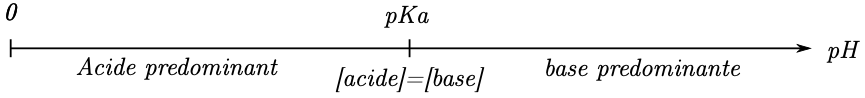
\includegraphics[scale=.5]{figures/acide_base/diag_predominance}

\etiquette{Application}: Réaliser les diagrammes de prédominance des couples suivants :\\
\textbf{Dans la famille : acide carboxylique/ion carboxylate} : $\rm{RCOOH/RCOO^-}$\\
Exemple de l'acide méthanoïque de pKa égal à 3,8.\\
\textbf{Dans la famille : amine/ion ammonium} : $\rm{RNH_3^+/RNH_2}$\\
Exemple de la méthylamine de pKa égal à 10,6.\\
Exemple de la diméthylamine de pKa égal à 10,8

\subsection*{Le cas des acides $\alpha$aminés}
La valine est un acide $\alpha$aminé. L'une de ses formes acido-basiques est la suivante :\\
\chemfig{CH(-[2]CH_3)(-[4]H_3C)-CH(-[2]CO_2H)-NH_3^+}\\

On lui attribue deux pKa : 2,3 et 9,7.
\begin{enumerate}
\item Entourer les groupes caractéristiques de la valine qui possèdent des propriétés acido-basiques.
\item Quel groupe caractéristique est responsable du pKa le plus petit ? le plus grand ?
\item Ecrire les 4 formes de la valine théoriquement possibles.
\item Tracer le diagramme de prédominance de la valine en fonction du pKa égal à 2,3.
\item Sous ce diagramme, tracer le diagramme de prédominance en fonction du pKa égal à 9,7.
\item En étudiant les diagrammes tracés précédemment, montrer que l'une des formes trouvées à la question 3 n'existe pas.
\item La valine est abondante dans le blanc d'\oe uf, dont le pH est voisin de 7,5. Sous quelle forme acido-basique trouve-t-on majoritairement la valine dans le blanc d'\oe uf ?
\end{enumerate}


\subsection{Diagramme de distribution}
\begin{minipage}{0,6\linewidth}
Le diagramme de distribution représente les pourcentages d'un acide et de sa base conjuguée en fonction de la valeur du pH. Il permet de connaître la composition d'un système à un instant donné.\\
Lorsque l'acide et sa base conjuguée sont en proportions égales, le pH est égal au \trou{pKa} du couple.
\end{minipage}
\begin{minipage}{0,4\linewidth}
\begin{center}
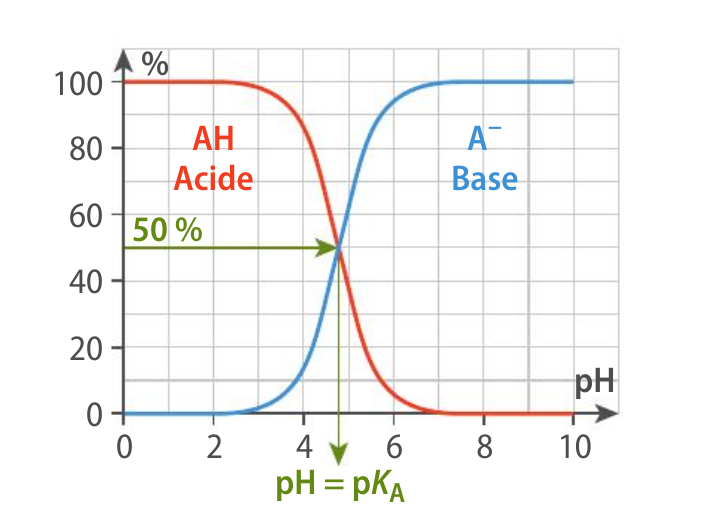
\includegraphics[scale=0.3]{figures/acide_base/fig_diag_distrib}
\end{center}

\end{minipage}

\subsection{Cas des indicateurs colorés}

Un indicateur coloré est une solution contenant un couple dont l'acide et la base conjuguée ont des teintes différentes. Sa zone de virage correspond à l'intervalle de pH dans lequel il passe d'une forme à l'autre. \\
\begin{center}
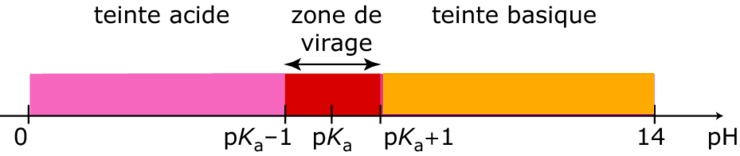
\includegraphics[scale=1.2]{figures/acide_base/fig_indic_color.jpg}
\end{center}

Un indicateur coloré peut être utilisé pour déterminer l'équivalence d'un titrage acide-base si le pH à l'équivalence se situe dans la zone de virage.

\section{Les solutions à connaître}
\subsection{Solution tampon}
\blocrouge{Définition}{
\trou{Une solution tampon est une solution dont le pH varie peu à l'ajout d'une petite quantité de base, d'acide ou d'eau}
}

Les solutions tampons permettent de contrôler la valeur du pH notamment lors de l'étalonnage d'un pH-mètre.

\subsection{Les petits basiques à connaître..}

\begin{tabular}{|c|p{5cm}|}
\hline
Nom de la solution&Formule chimique\\
\hline
acide chlorhydrique&\\
\hline
acide nitrique&\\
\hline
hydroxyde de sodium ou soude&\\
\hline
acide éthanoïque&\\
\hline
ammoniac&\\
\hline
\end{tabular}

\section*{Exercices à faire}

1 p 162
11, 14, 15 p 165
19 , 25 p 166-168

Bilan: 31 p 170

Type Bac: \url{https://www.labolycee.org/etude-de-lacide-benzoique-et-du-benzoate-de-sodium} Partie A
